\documentclass{beamer}
\usepackage{../tut-slides}
\usepackage{../mathoperatorsAuD}

\usepackage{lmodern}
\usepackage{amsmath,amssymb}
\usepackage{wasysym}
\usepackage{stmaryrd}
\usepackage{enumerate}
%\usepackage[inline]{enumitem} 		%customize label
%\newcommand{\labelitemi}{\raisebox{1pt}{\scalebox{.9}{$\blacktriangleright$}}}
%\newcommand{\labelitemii}{$\vartriangleright$}
%\newcommand{\labelitemiii}{--}
\setbeamertemplate{itemize item}{\raisebox{1pt}{\scalebox{.9}{$\blacktriangleright$}}}
\setbeamertemplate{itemize subitem}{$\vartriangleright$}

\usepackage{pgfplots}
\pgfplotsset{compat=1.10}   % in my packages used compat=1.15
\usepgfplotslibrary{fillbetween}
\usepackage{pgf}
\usepackage{tikz}
\usetikzlibrary{patterns,arrows, arrows.meta,calc,decorations.pathmorphing,backgrounds, positioning,fit,automata,shapes,matrix}
\usetikzlibrary{matrix}

\usepackage{booktabs}
\usepackage{tabularx}
\usepackage{tabu}
\newcommand*\head{\rowfont{\bfseries}}
\newcommand*{\tw}{\rowfont{\ttfamily}}
\renewcommand{\tabularxcolumn}[1]{>{\hspace{0pt}}m{#1}}
\usepackage{multirow}

\usepackage{cancel}

\usepackage{empheq}
\newcommand*\widefbox[1]{\fbox{\hspace{2em} #1 \hspace{2em}}}

\usepackage{tcolorbox}
\newtcolorbox{mymathbox}[1][]{colback=white, sharp corners, #1}

\usepackage{xcolor}
\usepackage{listings}
\usepackage{bold-extra}
\newcommand*{\ttfamilywithbold}{\fontfamily{lmtt}\selectfont}
\lstset{numbers=left, 
	numberstyle=\tiny, 
	breaklines=true,
	backgroundcolor=\color{cdgray!20},
	numbersep=5pt,
	language=C,
	tabsize=2,
	basicstyle=\footnotesize\ttfamilywithbold,
	showstringspaces=false} 

\lstdefinestyle{notebook}{
	basicstyle=\footnotesize\ttfamilywithbold,   
	breakatwhitespace=false,         
	breaklines=true,                 
	commentstyle=\itshape, 
	escapeinside={\%*}{*)},          % if you want to add LaTeX within your code
	extendedchars=true,              % lets you use non-ASCII characters; for 8-bits encodings only, does not work with UTF-8
	backgroundcolor=\color{cdgray!10},
	frame=single,
	keywordstyle=\bfseries,       % keyword style
	morekeywords={}, 
	language=C,                 % the language of the code
	numbers=left,                    % where to put the line-numbers; possible: (none, left, right)
	numbersep=5pt,                   
	numberstyle=\tiny\color{cdgray!50}, 
	rulecolor=\color{cddarkblue}, 
	tabsize=2,
	frameround=tttt
}

\newcommand{\col}[1]{\textcolor{cdpurple}{#1}}
\newcolumntype{R}[1]{>{\centering\arraybackslash}p{#1}}
\usepackage{tabularx}
\renewcommand{\tabularxcolumn}[1]{m{#1}}

\usepackage{qtree}
\usepackage[edges]{forest}
\usepackage{csquotes}

\begin{document}
	\title{Algorithmen und Datenstrukturen}
	\subtitle{Übung 10: Topologisches Sortieren \& Graphensuche}
	\author{Eric Kunze}
	\email{eric.kunze@tu-dresden.de}
	\city{TU Dresden}
%	\institute{Lehrstuhl für Grundlagen der Programmierung}
	\titlegraphic{
\includegraphics[width=2cm]{../TUD-white.pdf}}
	\date{\formatdate{13}{12}{2021}}

	\maketitle


%%%%%%%%%%%%%%%%%%%%%%%%%%%%%%%%%%%%%%%%%%%%%%%%%%%%%%%%%%%%%%%%%%%%%%%%%%%%%

\section{Topologisches Sortieren \\ \itshape Implementierung}

\begin{frame} \frametitle{Topologisches Sortieren}
	\small
	Gegeben sei ein gerichteter, azyklischer Graph $G = (V,E)$. Eine \textbf{topologische Sortierung} von $G$ ist eine \textit{bijektive} Abbildung $\operatorname{ord} \colon V \to \menge{1, \dots, \card{V}}$, sodass für alle $v, v' \in V$ mit $(v,v') \in E$ die Relation
	$\operatorname{ord}(v) < \operatorname{ord}(v')$ gilt.
	
	\textbf{Anschauung:} $\operatorname{ord}(v) = n \quad \leadsto \quad$ Knoten $v$ wird als $n$-tes Element gewählt (erhält Sortierungsnummer $n$) 
	
	\pause
	
	\textbf{Algorithmus:}
	
	\texttt{while} ( Elemente übrig ) 
	\begin{itemize}
		\item wähle Element $v$ ohne Vorgänger
		\item dekrementiere Anzahl der Vorgänger in den Nachfolgern von $v$
		\item füge $v$ der Ausgabeliste hinzu
		\item lösche $v$ aus $G$
	\end{itemize}
\end{frame}

\begin{frame}[fragile] \frametitle{Kodierungen}
	\small
	\begin{minipage}[t]{\dimexpr0.5\linewidth-\fboxrule-\fboxsep}
		\textbf{Kanten:} \\
		\lstinline|struct Edge { int from, to; };| 
		
		\begin{center}
			\scalebox{0.9}{%
				\begin{tikzpicture}[%
					>=stealth',
					semithick,
					every node/.style={font=\scriptsize},
					inbox/.style={anchor=mid, font=\small, align=center, pos=0.5},
					]
					\draw[thick, rounded corners=2pt, color=cdpurple] (0,0) rectangle ++(4,1);
					\node[anchor=west, color=cdpurple] (struct Edge) at (0.05, 1.25) {\texttt{struct Edge}};
					\draw (2,0) -- (2,1);
					\path (0,0) rectangle ++(2,1) node[inbox] (leftbox) {\texttt{from}} 
					rectangle ++(2, -1) node[inbox] (rightbox) {\texttt{to}};
			\end{tikzpicture}}
		\end{center}
		
		Bsp.: Kante $e = (3,5)$ \\
		\lstinline|struct Edge e = {3,5}| \\
		\lstinline|e.from == 3| \\
		\lstinline|e.to    == 5| \\	
		
		\onslide<3->{
			\textbf{Abbildung $\operatorname{ord}$:} Array \lstinline|int ord[]| mit $\operatorname{ord}(v) = j  \Leftrightarrow$ \texttt{ord[v] = j}
			\begin{itemize}
				\item initialisiert mit \texttt{-1}
			\end{itemize}
		}
	\end{minipage}
	\pause
	\begin{minipage}[t]{\dimexpr0.5\linewidth-\fboxrule-\fboxsep}
		\textbf{Graph:} Liste von Kanten \\
		$\leadsto$ \lstinline|struct Edge edges[];|
		
		\begin{center}
			\scalebox{0.9}{%
				\begin{tikzpicture}[%
					>=stealth',
					semithick,
					every node/.style={font=\scriptsize},
					inbox/.style={anchor=mid, font=\tiny, align=center, pos=0.5},
					]
					\foreach \x in {0,...,4}{
						\draw[thick, color=cdgreen] (\x, 0) rectangle ++ (1, 1);
						\draw[rounded corners=2pt, color=cdpurple] (\x + 0.1, 0.25) rectangle ++(0.8, 0.5);
						\draw (\x + 0.5, 0.25) -- (\x + 0.5, 0.75);}
					\node[anchor=west, color=cdgreen] (edges) at (0.05, 1.25) {\textcolor{cdpurple}{\texttt{struct Edge}} \texttt{edges}\textcolor{cdgreen}{\texttt{[]}}};
			\end{tikzpicture}}
		\end{center}
		
		Bsp.: Graph mit Kantenmenge $E = \menge{(1,2), (2,3), (3,1)}$
		\begin{center}
			\scalebox{0.8}{%
				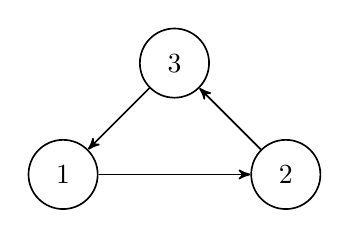
\begin{tikzpicture} [->, 
					>=stealth', 
					initial text=, 
					auto, 
					node distance=20mm, 
					bend angle=20, 
					semithick]%[node distance=2cm,auto]
					
					\node[state] (3) {$3$}; 
					\node[state] (2) [below right of=3] {$2$}; 
					\node[state] (1) [below left of=3] {$1$};
					
					\path[->]
					(1) edge (2) 
					(2) edge (3)
					(3) edge (1);
			\end{tikzpicture}}
		\end{center}

		$\leadsto$ \lstinline|struct Edge edges[] =| \\ \phantom{~} \hfill \lstinline|{{1,2}, {2,3}, {3,1}};| 
	\end{minipage}
\end{frame}

\begin{frame} \frametitle{Ein alternativer Algorithmus}
	\small
	\begin{minipage}[t]{\dimexpr0.5\linewidth-\fboxrule-\fboxsep}
		\texttt{while} ( Elemente übrig ) 
		\begin{itemize}
			\item wähle Element $v$ ohne Vorgänger
			\item dekrementiere Anzahl der Vorgänger in den Nachfolgern von $v$
			\item füge $v$ der Ausgabeliste hinzu
			\item lösche $v$ aus $G$
		\end{itemize}
	\end{minipage}
	\begin{minipage}[t]{\dimexpr0.5\linewidth-\fboxrule-\fboxsep}
		\texttt{for} jede Sortierungsnummer $j$
		\begin{itemize}
			\item \texttt{for} jeden Knoten	$v$
			\begin{itemize}
				\item teste ob $v$ gewählt werden kann, d.h. \\ noch nicht platziert ist \\ und eingehende Kanten bereits platziert
			\end{itemize}
			\item falls $v$ gewählt werden darf, setze \texttt{ord[v] = j}
		\end{itemize}
	\end{minipage}
\end{frame}

\begin{frame}[fragile] \frametitle{Aufgabe 1}
	\small
	\begin{lstlisting}[style=notebook, basicstyle=\scriptsize\ttfamilywithbold]
void topsort(int n, int e, struct Edge edges[], int ord[]) {
	int j = 1, node, edge, ok;
	while (j <= n) 	{
		for (node = 0; node < n; ++node) {
			if (ord[node] == -1) {
				ok = 1;
				for (edge = 0; edge < e; ++edge) {
					if (edges[edge].to == node &&
							ord[edges[edge].from] == -1)
						ok = 0;
				}
				if (ok) {
					ord[node] = j;
					j++;
					break;
				}
			}
		}
	}
}
	\end{lstlisting}
\end{frame}

\begin{frame}[fragile] \frametitle{Ein Beispiel}
	\small
	\begin{minipage}{\dimexpr0.5\linewidth-\fboxrule-\fboxsep}
		\begin{center}
			\scalebox{0.8}{%
				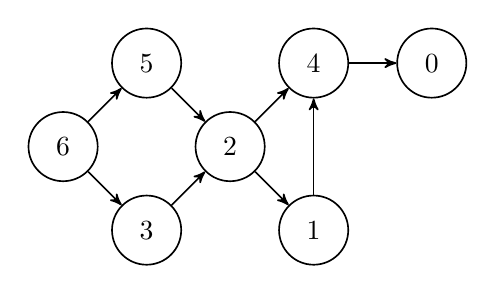
\begin{tikzpicture} [->, 
					>=stealth', 
					initial text=, 
					auto, 
					node distance=15mm, 
					bend angle=20, 
					semithick]%[node distance=2cm,auto]
					
					\node[state] (6) {$6$}; 
					\node[state] (5) [above right of=6] {$5$}; 
					\node[state] (3) [below right of=6] {$3$};
					\node[state] (2) [below right of=5] {$2$};
					\node[state] (4) [above right of=2] {$4$};
					\node[state] (1) [below right of=2] {$1$};
					\node[state] (0) [right       of=4] {$0$};
					
					\path[->]
					(6) edge (5) 
					(6) edge (3)
					(5) edge (2)
					(3) edge (2)
					(2) edge (4)
					(2) edge (1)
					(1) edge (4)
					(4) edge (0);
			\end{tikzpicture}}
		\end{center}
	\end{minipage}
	\pause
	\begin{minipage}{\dimexpr0.5\linewidth-\fboxrule-\fboxsep}
		Knoten 6 bekommt Nummer 1. \\
		Knoten 3 bekommt Nummer 2. \\
		Knoten 5 bekommt Nummer 3. \\
		Knoten 2 bekommt Nummer 4. \\
		Knoten 1 bekommt Nummer 5. \\
		Knoten 4 bekommt Nummer 6. \\
		Knoten 0 bekommt Nummer 7. 		
	\end{minipage}
	
	\bigskip
	\centering \pause
	
	\scalebox{1}{%
		\begin{tabular}{r|ccccccc}
			\hline
			$v =$ & 0 & 1 & 2 & 3 & 4 & 5 & 6 \\
			\hline
			$\operatorname{ord}(v) =$ & 7 & 5 & 4 & 2 & 6 & 3 & 1 \\
			\hline
	\end{tabular}} 
	
	\bigskip
	
	\texttt{ord = [7, 5, 4, 2, 6, 3, 1]}
	
\end{frame}

%%%%%%%%%%%%%%%%%%%%%%%%%%%%%%%%%%%%%%%%%%%%%%%%%%%%%%%%%%%%%%%%%%%%%%%%%%%%%%%%%%%

\section{Breiten- und Tiefensuche}

\begin{frame}[t] \frametitle{Suchverfahren}
	\begin{itemize}
		\item Ziel: Finden eines Knotens mit bestimmter Beschriftung in einem Graphen
		\item hier: uninformierte Suche mit Tiefen- und Breitensuche
	\end{itemize}

	\bigskip 
	
	\begin{center}
		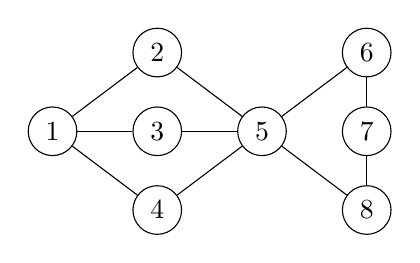
\begin{tikzpicture}
			\node [circle,draw] (1) at (-1.33,0)  {$1$};
			\node [circle,draw] (2) at (0,1)  {$2$};
			\node [circle,draw] (3) at (0,0) {$3$};
			\node [circle,draw] (4) at (0,-1) {$4$};
			
			\node [circle,draw] (5) at (1.33,0)  {$5$};
			
			\node [circle,draw] (6) at (2.66,1)  {$6$};
			\node [circle,draw] (7) at (2.66,0)  {$7$};
			\node [circle,draw] (8) at (2.66,-1) {$8$};
			
			% Kanten
			% \path (1) -- node[weight] {$3$} (3)
			\draw (1) -- (2);
			\draw (1) -- (3);
			\draw (1) -- (4);
			
			\draw (2) -- (5);
			\draw (3) -- (5);
			\draw (4) -- (5);
			\draw (5) -- (6);
			\draw (6) -- (7);
			\draw (7) -- (8);
			\draw (5) -- (8);
		\end{tikzpicture}
	\end{center}	
\end{frame}

\begin{frame}[t] \frametitle{Tiefensuche}
    \begin{itemize}
    	\item gehe in die Tiefe: \\
    	\enquote{entdecke erst Kinder, dann Geschwister}
    	\item Datenstruktur: Keller
    	\item Nachfolger werden \emph{oben} auf den Keller gelegt
    	\item nächster Knoten wird \emph{oben} vom Keller genommen
    \end{itemize}
	
	\bigskip 
	
	\textbf{Keller:}
	\begin{center}
		\begin{tikzpicture}[scale=0.5]
			\draw[thick] (-1,-1) -- (3,-1);
			\foreach \y in {0,...,5}
				\draw (0,\y) rectangle ++(2,-1);
			\node[anchor=north east] (nachfolger) at (-3,5) {Nachfolger};
			\draw[->, arrows=-Stealth, bend angle=45, bend left]  (nachfolger) to (1,5);
			\node[anchor=south west] (next) at (4,4) {nächster Knoten};
			\draw[->, arrows=-Stealth]  (2,4.5) to (next);
		\end{tikzpicture}
	\end{center}
\end{frame}

\begin{frame}[t] \frametitle{Breitensuche}
    \begin{itemize}
    	\item gehe in die Breite: \\
    	\enquote{entdecke erst Geschwister, dann Kinder}
    	\item Datenstruktur: Warteschlange
    	\item Nachfolger stellen sich \emph{hinten} an
    	\item nächster Knoten wird von \emph{vorn} genommen
    \end{itemize}

	\bigskip 
	
	\textbf{Warteschlange:}
	\begin{center}
		\begin{tikzpicture}[scale=0.5]
			\foreach \x in {0,...,5}
			\draw[color=cddarkblue] (\x,0) rectangle ++(1,1);
			\node[anchor=south west] (nachfolger) at (9,1) {Nachfolger};
			\draw[->, arrows=-Stealth, bend angle=45, bend right]  (nachfolger.west) to (6.5,1);
			\node[anchor=north] (next) at (-1.5,-1) {nächster Knoten};
			\draw[->, arrows=-Stealth, bend angle=45, bend right]  (0,0.5) to (next.north);
		\end{tikzpicture}
	\end{center}
\end{frame}

\begin{frame} \frametitle{Verallgemeinerte Graphensuche}
	\small
	\textbf{Beobachtung}: Suche läuft ähnlich ab
	\begin{itemize}
		\item Operation 1: Lesen des nächsten Knotens \hfill \texttt{READ}
		\item Operation 2: Löschen des gewählten Knotens \hfill \texttt{REMOVE}
		\item Operation 3: Hinzufügen eines Nachfolgerknotens \hfill \texttt{INSERT}
		\item Operation 4: Leerheit der Datenstruktur \hfill \texttt{EMPTY}
	\end{itemize}

	\pause
	\begin{center}
		\begin{tabular}{l|ccccc}
			& \texttt{STORAGE} & \texttt{READ} & \texttt{REMOVE} & \texttt{INSERT} & \texttt{EMPTY} \\ \hline
			Tiefensuche & Keller & \texttt{top} & \texttt{pop} & \texttt{push} & \texttt{empty} \\
			Breitensuche & Queue & \texttt{head} & \texttt{dequeue} & \texttt{enqueue} & \texttt{nil} \\
		\end{tabular}
	\end{center}
	
	\pause
	weitere Möglichkeit für \texttt{STORAGE}: \textbf{Prioritätswarteschlange} \\
	{\scriptsize (vgl. Übung 11, Dijkstra-Algorithmus für kürzeste Wege in gewichteten Graphen)}
	\begin{itemize}
		\item Wahl des nächsten Elementes anhand eines Prioritätswertes
		\item Vorstellung: \textit{geordnete} Warteschlange
	\end{itemize}
\end{frame}

\begin{frame} \frametitle{Aufgabe 2}
	\centering
	\begin{minipage}{\dimexpr0.5\linewidth-\fboxrule-\fboxsep}
		\begin{center}
			\scalebox{1}{%
			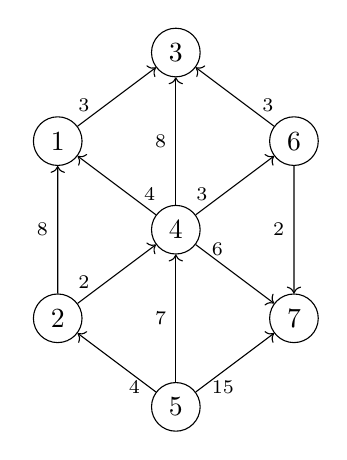
\begin{tikzpicture}[scale=1.5]
				% Knoten
				\node (4) at (0,0)  [circle,draw] {4};
				\node (3) at (0,1.5)  [circle,draw] {3};
				\node (5) at (0,-1.5) [circle,draw] {5};
				\node (1) at (-1,.75) [circle,draw] {1};
				\node (2) at (-1,-.75) [circle,draw] {2};
				\node (6) at (1,.75) [circle,draw] {6};
				\node (7) at (1,-.75) [circle,draw] {7};
				% Kanten
				\tikzset{every node/.style={font=\scriptsize}}
				%		\path (1) -> node[weight] {$3$} (3)
				\draw[->] (1) edge node[pos=.08, above]{3} (3);
				\draw[->] (2) edge node[left] {8} (1);
				\draw[->] (2) edge node[pos=.08, above]{2} (4);
				\draw[->] (4) edge node[left] {8} (3);
				\draw[->] (4) edge node[pos=.08, above]{4} (1);
				\draw[->] (4) edge node[pos=.08, above]{3} (6);
				\draw[->] (4) edge node[pos=.08, right]{6} (7);
				\draw[->] (5) edge node[pos=.08, left]{4} (2);
				\draw[->] (5) edge node[left] {7} (4);
				\draw[->] (5) edge node[pos=.08, right]{15} (7);
				\draw[->] (6) edge node[pos=.08, above]{3} (3);
				\draw[->] (6) edge node[left] {2} (7);
		\end{tikzpicture}}
		\end{center}
	\end{minipage}
	\begin{minipage}{\dimexpr0.5\linewidth-\fboxrule-\fboxsep}
		\begin{enumerate}[(a)]
			\item \textbf{Tiefensuche}: \\ 3 verschiedene depth-first trees 
			\item \textbf{Breitensuche}: \\ 3 verschiedene breadth-first trees
		\end{enumerate}
	\end{minipage}
\end{frame}

\begin{frame} \frametitle{Aufgabe 2 --- Teil (a)}
    \textbf{Tiefensuche}

	Es gibt $5$ verschiedene depth-first-trees, z.B.:

	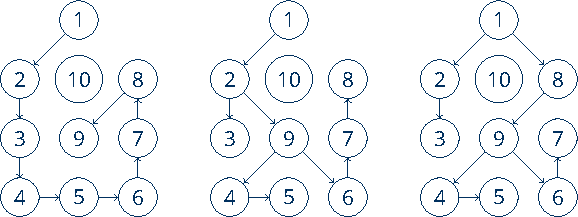
\includegraphics[width=\linewidth]{./tut11_task2-dft.pdf}
\end{frame}

\begin{frame} \frametitle{Aufgabe 2 --- Teil (b)}
    \textbf{Breitensuche}

	Es gibt $5$ verschiedene breadth-first-trees, z.B.:

	\begin{center}
		\begin{tikzpicture}
			% Knoten
			\node (1) at (1,0)  [circle,draw] {1};
			\node (2) at (0,-1) [circle,draw] {2};
			\node (3) at (0,-2) [circle,draw] {3};
			\node (4) at (0,-3) [circle,draw] {4};
			\node (5) at (1,-3) [circle,draw] {5};
			\node (6) at (2,-3) [circle,draw] {6};
			\node (7) at (2,-2) [circle,draw] {7};
			\node (8) at (2,-1) [circle,draw] {8};
			\node (9) at (1,-2) [circle,draw] {9};
			\node (10) at (1,-1) [circle,draw] {10};
			% Kanten
			\tikzset{every node/.style={color=cdgray, font=\tiny}}
%			\path[->] (1) edge node {${a}, {C} \mapsto {D}$} (2);
			\path[->] (1) edge node[left] {1} (2);
			\path[->] (2) edge node[left] {2} (3);
			\path[->] (3) edge node[left] {3} (4);
			\path[->] (4) edge node[above] {5} (5);
			\path[->] (9) edge node[left] {4} (6);
			\path[->] (6) edge node[right] {6} (7);
			\path[->] (1) edge node[right] {1} (8);
			\path[->] (2) edge node[left] {2} (9);
		\end{tikzpicture}		
		\hspace{2em} \pause
		\begin{tikzpicture}
			% Knoten
			\node (1) at (1,0)  [circle,draw] {1};
			\node (2) at (0,-1) [circle,draw] {2};
			\node (3) at (0,-2) [circle,draw] {3};
			\node (4) at (0,-3) [circle,draw] {4};
			\node (5) at (1,-3) [circle,draw] {5};
			\node (6) at (2,-3) [circle,draw] {6};
			\node (7) at (2,-2) [circle,draw] {7};
			\node (8) at (2,-1) [circle,draw] {8};
			\node (9) at (1,-2) [circle,draw] {9};
			\node (10) at (1,-1) [circle,draw] {10};
			% Kanten
			\tikzset{every node/.style={color=cdgray, font=\tiny}}
			\draw[->] (1) edge node[left] {1} (2);
			\draw[->] (2) edge node[left] {2} (3);
			\draw[->] (2) edge node[left] {2} (9);
			\draw[->] (9) edge node[left] {3} (4);
			\draw[->] (4) edge node[above] {4} (5);
			\draw[->] (9) edge node[left] {3} (6);
			\draw[->] (6) edge node[right] {5} (7);
			\draw[->] (1) edge node[right] {1} (8);
		\end{tikzpicture}
		\hspace{2em} \pause	
		\begin{tikzpicture}
			% Knoten
			\node (1) at (1,0)  [circle,draw] {1};
			\node (2) at (0,-1) [circle,draw] {2};
			\node (3) at (0,-2) [circle,draw] {3};
			\node (4) at (0,-3) [circle,draw] {4};
			\node (5) at (1,-3) [circle,draw] {5};
			\node (6) at (2,-3) [circle,draw] {6};
			\node (7) at (2,-2) [circle,draw] {7};
			\node (8) at (2,-1) [circle,draw] {8};
			\node (9) at (1,-2) [circle,draw] {9};
			\node (10) at (1,-1) [circle,draw] {10};
			% Kanten
			\tikzset{every node/.style={color=cdgray, font=\tiny}}
			\draw[->] (1) edge node[left] {1} (2);
			\draw[->] (2) edge node[left] {3} (3);
			\draw[->] (1) edge node[right] {1} (8);
			\draw[->] (8) edge node[right] {2} (9);
			\draw[->] (9) edge node[left] {4} (4);
			\draw[->] (9) edge node[left] {4} (6);
			\draw[->] (4) edge node[above] {5} (5);
			\draw[->] (6) edge node[right] {6} (7);
		\end{tikzpicture}
	\end{center}
\end{frame}

%%%%%%%%%%%%%%%%%%%%%%%%%%%%%%%%%%%%%%%%%%%%%%%%%%%%%%%%%%%%%%%%%%%%%%%%%%%%%%%%%%%

\end{document}